
\usetikzlibrary{shapes,arrows}

\newcommand{\hoo}[0]{H_2O}

\tikzstyle{decision} = [diamond, draw, fill=blue!30, text badly centered, node distance=3.5cm, inner sep=3pt,  rounded corners]
    
    %  text width=15em
\tikzstyle{block} = [inner sep = 10,rectangle, draw, fill=black!10, text centered, rounded corners, minimum height=3em,node distance=2cm]
    
\tikzstyle{line} = [draw, -latex']

\tikzstyle{cloud} = [draw, rectangle,fill=orange!40, node distance=5cm,
    minimum height=2em]












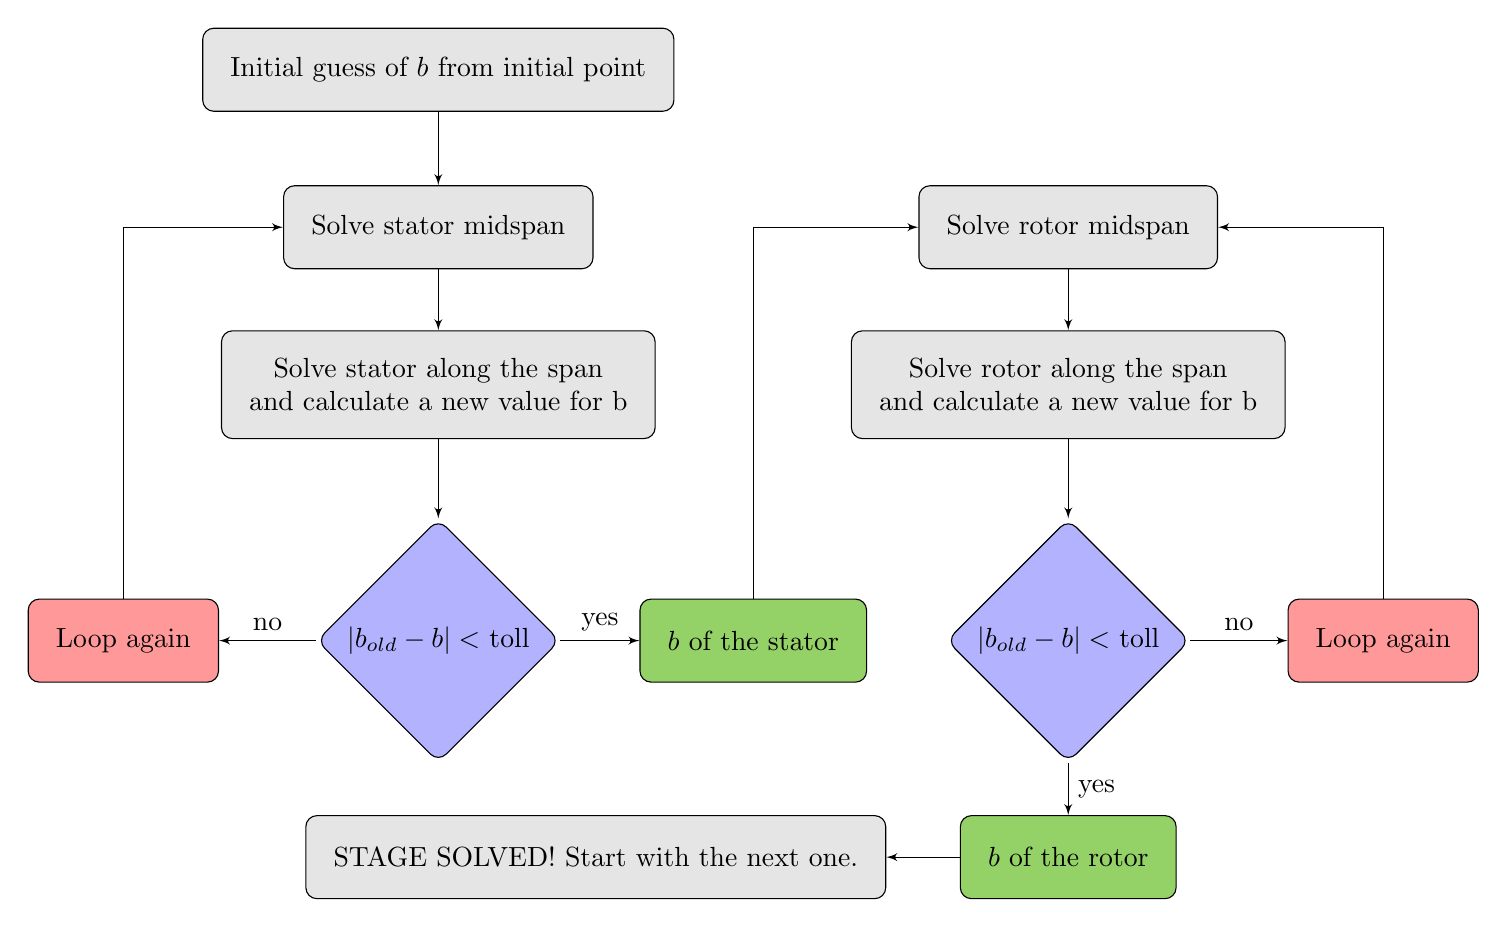
\begin{tikzpicture}
%[node distance = 1cm, auto]

\node [block,align=center] (start) {Initial guess of $b$ from initial point};

\node [block, align=center, below of = start] (calculation1){Solve stator midspan};
\node [block, align=center, below of = calculation1] (calculation2) {Solve stator along the span\\and calculate a new value for b};
\node [decision, below of=calculation2 ,align=center, node distance=3.25cm] (decide) {$ |b_{\text{old}} - b |< $ toll};
    
\node [block,node distance=4cm,fill=red!40, left of=decide,align=center] (no) {Loop again};
\node [block,node distance=4cm,fill=green!40!olive!60, right of=decide,align=center] (yes) {$b$ of the stator};



\node [block, align=center, right of = calculation1,node distance=8cm] (calculation21){Solve rotor midspan};
\node [block, align=center, below of = calculation21] (calculation22) {Solve rotor along the span\\and calculate a new value for b};
\node [decision, below of=calculation22 ,align=center, node distance=3.25cm] (decide2) {$ |b_{\text{old}} - b |< $ toll};
\node [block,node distance=4cm,fill=red!40, right of=decide2,align=center] (no2) {Loop again};
\node [block,node distance=2.75cm,fill=green!40!olive!60, below of=decide2,align=center] (yes2) {$b$ of the rotor};
\node [block, align=center, left of = yes2, node distance=6cm] (final){STAGE SOLVED! Start with the next one.};

% now we link together the blocks with arrows

\path [line] (start) -- (calculation1);
\path [line] (calculation1) -- (calculation2);
\path [line] (calculation2)--(decide);
\path [line] (decide) -- node[anchor=south] {yes} (yes);
 \path [line] (decide) -- node[anchor=south] {no} (no);
 \path [line] (no) |- (calculation1) ;
 
 \path [line] (yes) |- (calculation21) ;
 
\path [line] (calculation21) -- (calculation22);
\path [line] (calculation22)--(decide2);
\path [line] (decide2) -- node[anchor=west] {yes} (yes2);
 \path [line] (decide2) -- node[anchor=south] {no} (no2);
 \path [line] (no2) |- (calculation21) ;
\path [line] (yes2) -- (final);
% 
% \path[line] (c_and_m) --  (dadN) ;
% \path[line] (N) --  (update) ;

\end{tikzpicture}